\documentclass[conference]{IEEEtran}
\IEEEoverridecommandlockouts
% The preceding line is only needed to identify funding in the first footnote. If that is unneeded, please comment it out.
 
\usepackage{amsmath,amssymb,amsfonts}
\usepackage{algorithmic}
\usepackage{graphicx} 
\usepackage{textcomp}
\usepackage{xcolor} 
\usepackage[backend=biber]{biblatex}
\addbibresource{main.bib}

 \def\BibTeX{{\rm B\kern-.05em{\sc i\kern-.025em b}\kern-.08em
     T\kern-.1667em\lower.7ex\hbox{E}\kern-.125emX}}
    
\begin{document}
 
  
\title{Earth at night*\\
{\footnotesize \textsuperscript{*}The visualisation of average radiance in specific area}
}
 
\author{\IEEEauthorblockN{1\textsuperscript{st} Zhen Chen}
\IEEEauthorblockA{\textit{Faculty of Computing and Mathematical Sciences} \\
\textit{The University of Waikato}\\
Beijing, China \\
1561010}
\and
\IEEEauthorblockN{2\textsuperscript{nd} Huajie Xu}
\IEEEauthorblockA{\textit{dept. name of organization (of Aff.)} \\
\textit{name of organization (of Aff.)}\\
City, Country \\
email address or ORCID}
\and
\IEEEauthorblockN{3\textsuperscript{rd} Shengzhu Wang}
\IEEEauthorblockA{\textit{dept. name of organization (of Aff.)} \\
\textit{name of organization (of Aff.)}\\
City, Country \\
email address or ORCID}
\and
\IEEEauthorblockN{4\textsuperscript{th} Wenjie Tong}
\IEEEauthorblockA{\textit{dept. name of organization (of Aff.)} \\
\textit{name of organization (of Aff.)}\\
City, Country \\
email address or ORCID}
\and
\IEEEauthorblockN{5\textsuperscript{th} SiXiang Xiong}
\IEEEauthorblockA{\textit{dept. name of organization (of Aff.)} \\
\textit{name of organization (of Aff.)}\\
City, Country \\
email address or ORCID}
}

\maketitle

\begin{abstract}
This document is the description about the solution for Assignment 2 of Compx527 paper 
in Waikato University. World Bank Nightime Light Data consists of a lot of satellite imagery 
stored in Amazon Web Services (AWS). Recent files from 2012 to 2020 are generated by the sensor 
named Visible Infrared Imaging Radiometer Suite Day-Night Band (VIIRS DNB) \cite{WorldBan13:online}. All these things are 
stored by Cloud Optimized GeoTIFF (COG) \cite{CloudOpt5:online} format and organized by Spatial Temporal Asset Catalog (STAC) standard \cite{SpatioTe90:online}. 
This project only need the imagery in 3 specific areas, but it is neccessary to process all of them. 
From them, you can learn the trend of their radiance in the period. It is also a good chance to have a better understanding of ecnomic trend by them.
Some researchers also try to find the light pollution by this kind of data \cite{BARA2020106658}.
\end{abstract}

\begin{IEEEkeywords}
Night light, STAC, COG, VIIRS DNB, AWS
\end{IEEEkeywords}

\section{Solution Summary}
A lot of services are depended by this project. It is important to know that imagery from AWS open datasets 
has almost not processed too much before being stored. So the Geospatial Data Abstraction Library (GDAL) is 
imported for the complicated computing. GDAL is a common open source library used for various geospatial data formats \cite{GDAL—GDA74:online}. 
In this project, it is the translator from raster file to vector. So that it is possible to calculate the insection area 
between the satellite imagery and the target area. All of the imagery is the orignal file from the satellite, so
the bad weather would impact the real data, i.e. cloudy and some other atmosphere issues. The project objective is 
to learn the AWS usage and security practice, to get more real data as the reality, more research on how to identify 
cloud and bad weather still need to be done. These bad cases would be influence this project demo very obivously.

In addition, to ensure the development schedule, Lark, which is a kind of instant messenger used in Chinese office, 
is used to record documents and communicate in a group. At the first day, all team members were divided into 7 roles, i.e. project manager,
backend engineer, frontend engineer, devops, testing and data researcher. The project plan was made instantly when everybody understanding
the features, see Fig.~\ref{fig1}.

\begin{figure}[htbp]
    \centerline{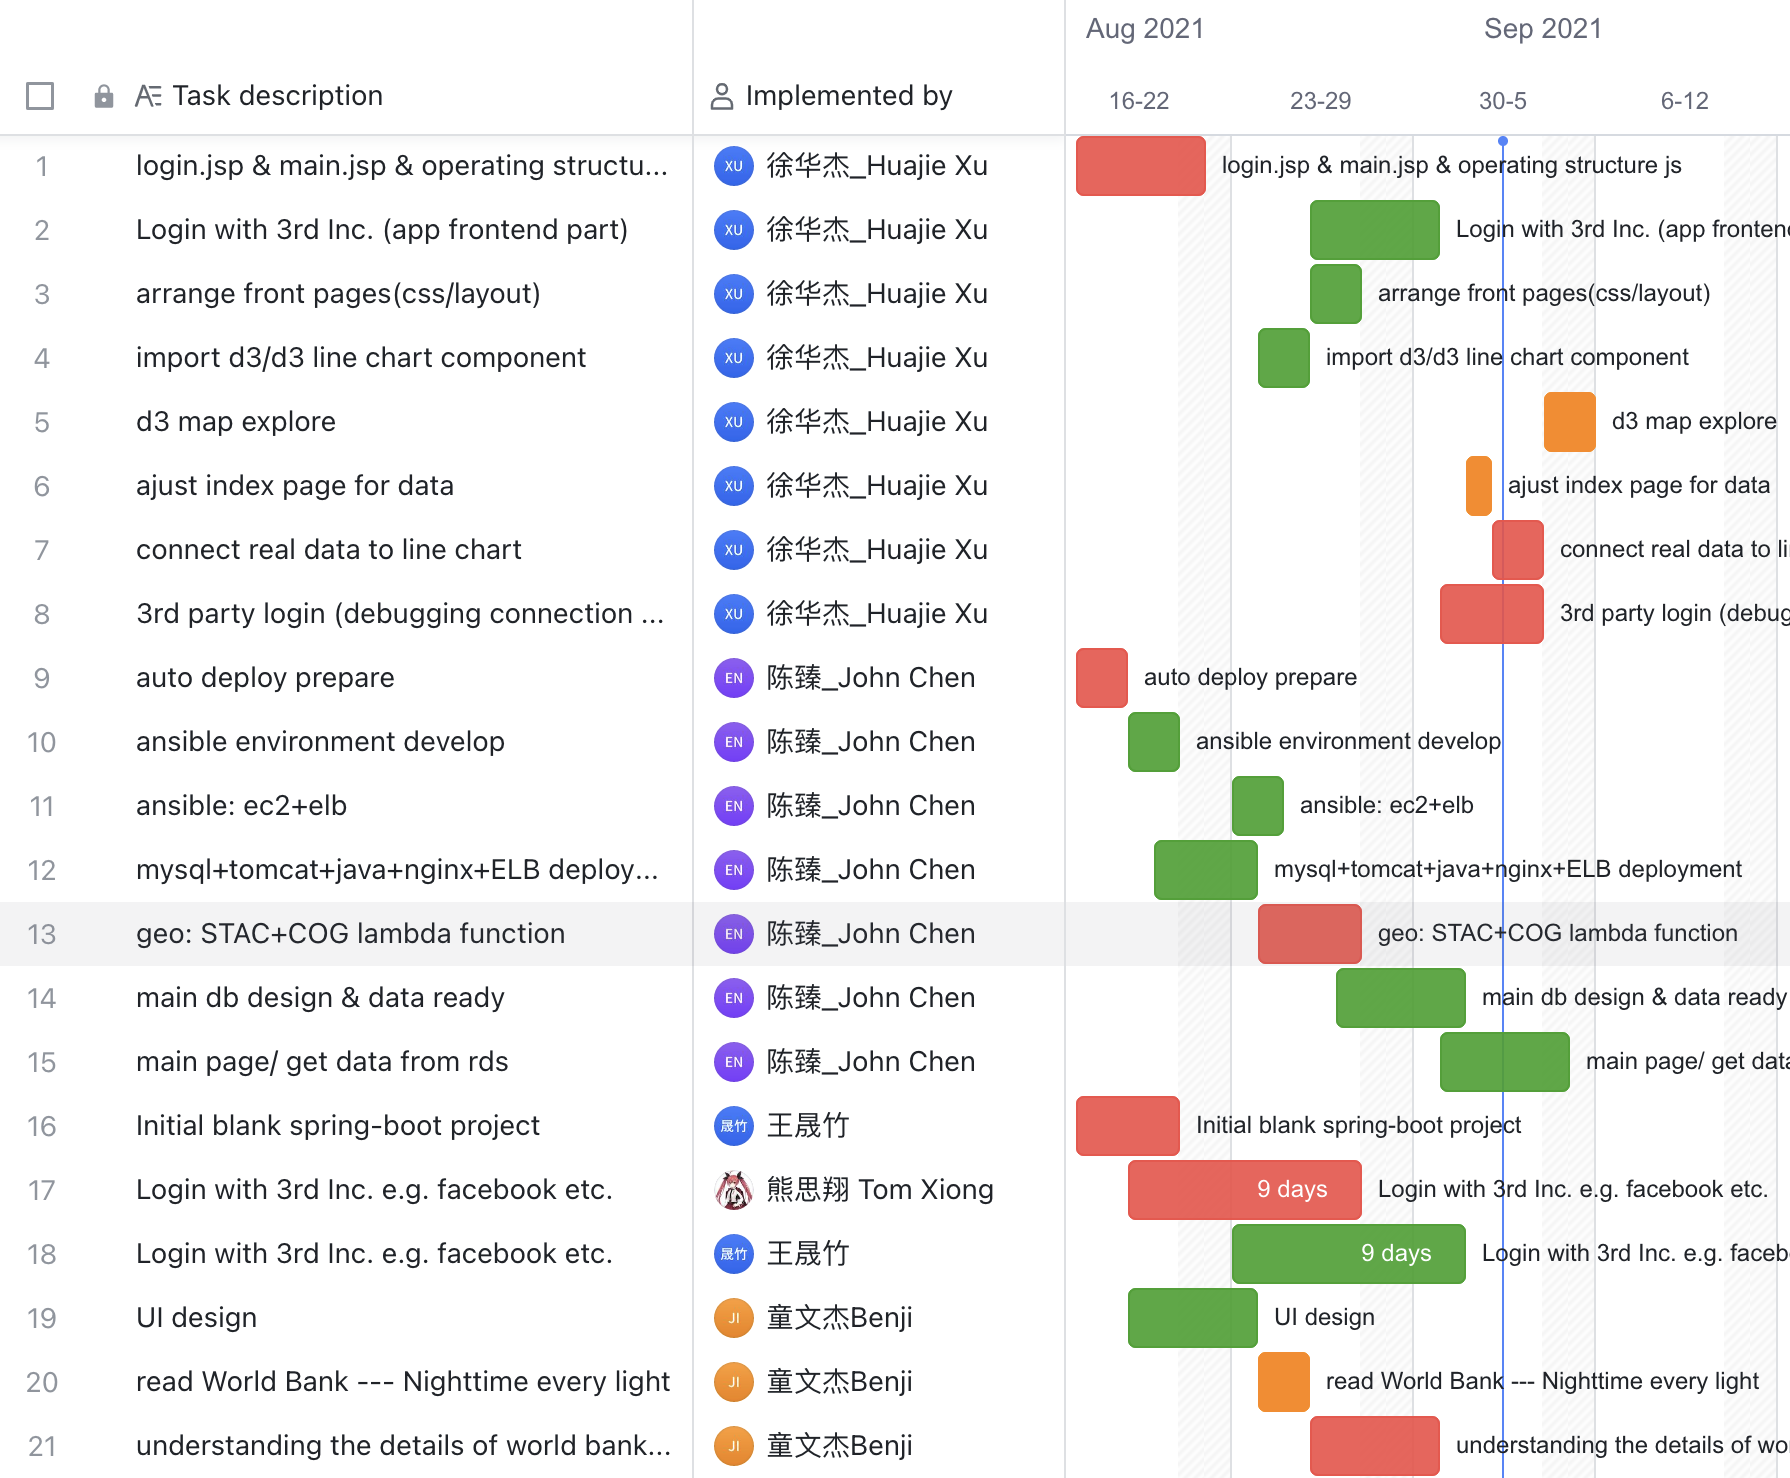
\includegraphics[width=260pt]{images/plan.png}}
    \caption{Project schedule}
    \label{fig1}
\end{figure}

Agile development project management method was used in this project. So the team has a short video meeting everyday. This plan is the last 
result after several development iterations.

The architecture of our solution is shown as Fig.~\ref{fig2}. Both of security and budget are important. So a network address translation (NAT) gateway 
was used for the essential network design. But after two days, NAT had to close because of the budget alert. But it is neccessary that hiding the 
internal services into the internal network instead of exposing them to the internet.

There are two important methods to keep the passowrd safely. The first one is IAM role. IAM role provides good security protection in the whole structure.
Different IAM roles are generated to attach to different Lambda functions. The execution roles are granted permission of access to necessary AWS services. 
There are some common policies for them, e.g. AWSLambdaBasicExecutionRole and AmazonS3FullAccess policies. The second one is Secrets Manager service in AWS.
All of the passwords in this project are stored in it. Visiting it through Secrets Manager when needed.


\begin{figure}[htbp]
    \centerline{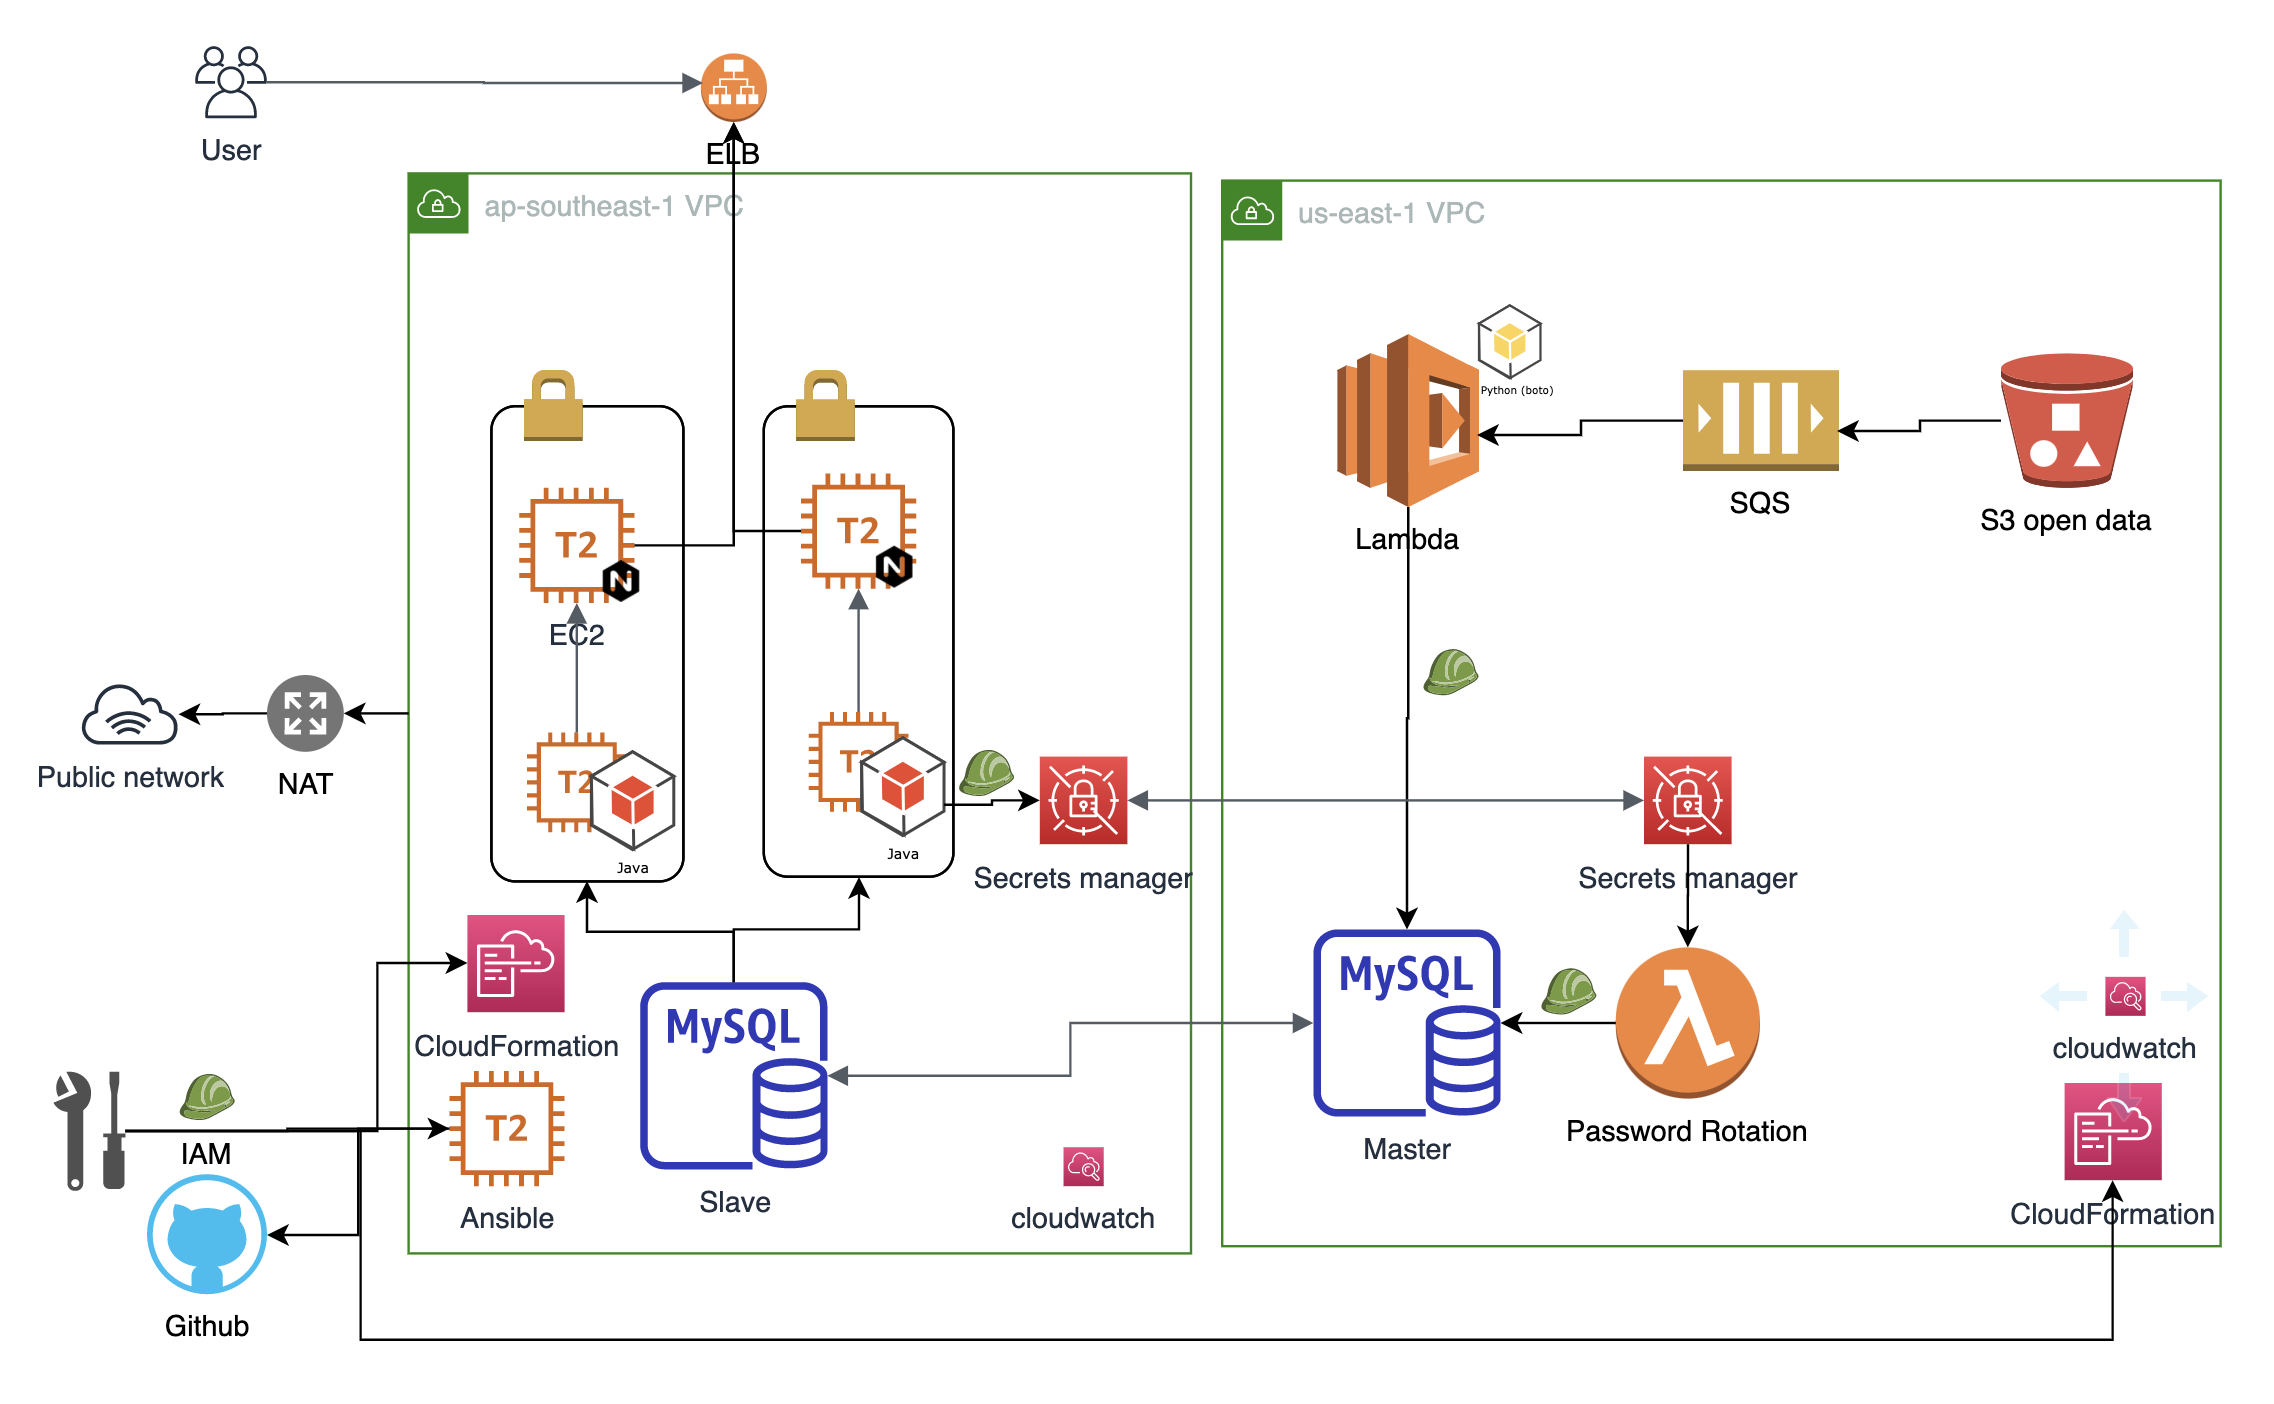
\includegraphics[width=260pt]{images/arch.png}}
    \caption{Architecture}
    \label{fig2}
\end{figure}
    
To process the S3 data, two Lambda functions are generated. One is to follow the STAC protcol to find the imagery, and another is to analyse pictures by GDAL, 
which is a kind of high cost computation in AWS. There are more than 4 pictures per day per area, and about 5,000 pictures per month totally. All the result processed by 
Lambda is stored in RDS and synced from us-east-1 region to ap-southeast-1 region. In addition, the password of MySQL is generated by a Lambda function and rotated 
timely. So the development team do not need to copy the password. Any features with passwords have to get it from Secrets Manager.  

When it comes to show the result in ap-southeast-1 region, network security is the most essential thing because this part of service can be touched by end users. 
So except ELB and the deployment server, there are not any other servers with public IP. All the EC2 instances can visit public network from the NAT, but public network 
can not visit them directly.

To explain more steps, there are some summaries as below. 

\subsection{Open Nighttime Lights}
this is the explaination  \cite{BARA2020106658}

\subsection{Frontend}
this is the explanation

\subsection{Vue}
this is the explanation

\subsection{D3}
this is the explanation
 
\subsection{Spring-boot}
this is the explanation

\subsection{Oauth github}
this is the explanation

\subsection{Ansible}
Ansible is a famous open source deployment platform, which is convenient to enable the infrastructure as code. 
It is the main tool to deploy most of the services in this project. Especially, a single EC2 instance with public 
IP is provided for it. But AWS service has to provision services by aws-cli instead of Ansible itself. There are still 
some libaries providing these functions but mostly are from external part.

\subsection{CloudFormation}
CloudFormation is a service in AWS, which can organize services very quickly and configure them by yaml or json. There area
several templates for provisioning different services. It is more convient than Ansible for some services. In this project, 
RDS and Lambda Services are dependent on it.

\subsection{Nginx/Tomcat}
Nginx is the widely used web server all over the world. It also has the excellent performance as a reverse proxy. 
Fontend server is the role in this project. Tomcat, which is behind Nginx, is a tranditional Java web container supporting 
Java Servlet. The visualisation is deisgned by Java and run in this container. Both Nginx and Tomcat are well-known because of 
the open source community and internet companies choosing.

\subsection{RDS/Lambda/Secrets Manager/SQS/EC2/NAT}
These items are names of services on AWS. Especially, Lambda are used to generate temperary password of RDS, and store it in 
Secrets Manager. It is really a good method to enhance the security for the password of database. On the other hand, NAT is a 
good feature for isolating the internal and external networks, but the price is too high to be used all the time in this project.

\section{Proposed solution}

A demo has finished all of tasks following the plan on time in this project. But to save budget, stoping NAT and processing parts of data are 
the temporary approaches. It is also possible to deal with the cloud and other disruption to ensure the accrute radiance value. All the 
other details are described as below.

\subsection{Whole infrastructure}
The main architecture is shown as Fig.~\ref{fig2}. 

\subsection{Frontend}

\subsection{Login}

\subsection{Data processing}

\subsection{Testing}

\subsection{Project management}

\section{Security Considerations}

\subsection{Networking}

\subsection{User}

\subsection{IAM}

\section{Team members and individual contribution within the team}
\begin{itemize}
    \item Zhen Chen:  PM, BE, DevOps
    \item Huajie Xu: FE
    \item Shengzhu Wang(Simon): BE
    \item SiXiang Xiong(Tom): BE, Testing
    \item Wenjie Tong: Data Researcher, Testing
\end{itemize}


\subsection{Figures and Tables}
 Use the abbreviation 
``Fig.~\ref{fig}'', even at the beginning of a sentence.

\begin{table}[htbp]
\caption{Table Type Styles}
\begin{center}
\begin{tabular}{|c|c|c|c|}
\hline
\textbf{Table}&\multicolumn{3}{|c|}{\textbf{Table Column Head}} \\
\cline{2-4} 
\textbf{Head} & \textbf{\textit{Table column subhead}}& \textbf{\textit{Subhead}}& \textbf{\textit{Subhead}} \\
\hline
copy& More table copy$^{\mathrm{a}}$& &  \\
\hline
\multicolumn{4}{l}{$^{\mathrm{a}}$Sample of a Table footnote.}
\end{tabular}
\label{tab1}
\end{center}
\end{table}

\begin{figure}[htbp]
\centerline{
\includegraphics{fig1.png}}
\caption{Example of a figure caption.}
\label{fig}
\end{figure}
 

 
\printbibliography

\end{document}
